\documentclass[UTF8]{article}
\usepackage{graphicx}
\usepackage{setspace}
% \usepackage{ctex}
\usepackage{amsmath}
\usepackage{geometry}


\newtheorem{thm}{Theorem}
\newtheorem{def}{Definition}
\newtheorem{lemma}{Lemma}
\newtheorem{pf}{Proof}
\newtheorem{algorithm}{Algorithm}


% \geometry{a4paper,left=2cm,right=2cm,top=1cm,bottom=1cm}
% \setstretch{1.5}
\geometry{a4paper,scale=0.8}
\renewcommand{\baselinestretch}{1.5}

\title{An example of unbalanced cooperative games:Machine Scheduling Game}
\author{Dis\cdot count}
% \date{Feb 2019}
\begin{document}

\maketitle{}

\section{Basic concept}

At first, we will introduce some preparatory knowledge as follows. A cooperative game model of transferable utility can be described as a pair of parameters $(V,c)$, among which $V={1,2,\dots,v}$ represents the set of $v \geq 2$ players and $c:2^{V}\to \mathbb{R}$ is a characteristic function. A coalition is defined as a nonempty subset of players, with the grand coalition $V$. Meanwhile, we use $S=2^{V} \setminus\{\emptyset\}$ to represent the set of all coalitions. For each coalition $s\in S$, characteristic function $c(s)$ means the minimum cost when the players in coalition $s$ cooperate to finish their work.
We use the vector $\alpha=[\alpha_{1},\alpha_{2},\dots,\alpha_{v}] \in \mathbb{R}^{v}$ to indicate the cost allocation in cooperative games, and $\alpha_{k}$ stands for the cost that the player $k \in V$ need to bear.
Now that we express the cost allocation of any player $k \in V$ as $\alpha_{k}$, we can use $\alpha(s)=\sum_{k\in{s}}\alpha_{k}$ to denote the total cost of every coalition $s\in S$.
The most important concept in cooperative game is the core, which is denoted as $Core(V,c)$. That is, the set of the cost allocation vectors $\alpha\in\mathbb{R}^{v}$ which satisfy the balance budget restriction $\alpha(V)=c(V)$ and coalition stability restriction $\alpha(s) \leq c(s)$. In other words, we have the following definition: $Core(V,c)= \left\{\alpha:\alpha(V)=c(V), \alpha(s)\leq c(s)\ \text{for all}\ s \in S \setminus\{V\}, \alpha \in \mathbb{R}^{v} \right\}$.
Usually in order to stabilize the grand coalition, that is to say, let the total cost induced by all the players be less than $c(V)$, the authority will adopt the subsidy policy to the players in the grand coalition.
The required minimum subsidy can be expressed as:
\begin{equation} \label{model}
  \omega^*=\mathop{\min}_{\alpha}\{c(V)-\alpha(V):\alpha(s)\leq c(s)\ \text{对所有}\ s \in S, \alpha\in\mathbb{R}^{v}\}
\end{equation}
In order to demonstrate the impact of pricing(taxation) on subsidy, we define the characteristic function as follow.
\[
c(s)=\mathop{\min}\{cx+Pm:Ax \geq By^s+D, \tilde{alpha}x \leq m,x \in \mathbb{Z} ,m \in \mathbb{Z}\} ,\text{and} s \in S
\]

P represents the price of public facilities and M is the number of public facilities. Meanwhile, we divide $c(s)$ into two parts: one is called as time cost $c_0(s) = cx$ which is the function of processing time, and the other is facility cost $Pm$.

Our aim is to get the minimum cost that players in the grand coalition need to share at a given facility pricing. Our main interest is to stabilize the grand coalition by increasing pricing (taxation) as a subsidy. Before that, we will study how the facility pricing affects the value of subsidy.

We divide the formula (\ref{model}) as $c(s)=c_0(s)+m_sP, s \in S$, and as a common skill get its corresponding dual problem as follow:

\begin{equation} \label{dual}
  \omega(P)=\mathop{\max}_{\rho}\{c_0(V)+m_vP+\sum_{s\in S\setminus\{V\}}-\rho_s[c_0(s)+m_sP]:\sum_{s\in S\setminus\{V\}:k\in s}\rho_s=1,\forall k \in V,\rho_s\geq 0,\forall s \in S \setminus{V}\}
\end{equation}

For the formula (\ref{dual}), we can obtain that when $m_v $ is an integer, $\omega(P)$ is the pointwise maximum of a set of straight lines. That means $\omega(P) $ is convex during the corresponding interval, and the slope at $P$ is $m_v-\sum_{s\in S \setminus\{V\}} \rho_s \cdot m_s$.

According to the difinition, for any coalition $s\in S\setminus{V}$, we have the constraints $\alpha(s,P)\leq c(s)+m_sP$. Specially, we call the coalitions as the most unsatisfied coalitions which satisfy $\alpha(s,P)=c(s)+m_sP$. Simultaneously, we define $S^{\alpha P}=\{s_1^{\alpha P},s_2^{\alpha P},\dots,s_h(\alpha,P)^{\alpha P}\}$, which denotes the set of all unsatisfied coalitions, and $h(\alpha,P)=|S^{\alpha P}|$. From the above definition, we can obtain the following formula: $s_1^{\alpha P}\cup s_2^{\alpha P}\cup\dots\cup s_h(\alpha,P)^{\alpha P}=V$.
The formula shows that the set contains all the players, which reflects the equity in sharing cost.




\section{Summary for the machine scheduling game}
We will apply the cooperative theory on the machine schedule problem, and put it as a simple example to show our result.
We apply the proposed model to a parallel machine scheduling problem with unweighted jobs.
In such a machine scheduling game, each player$k$ has a job that needs to be processed on one of $m$ identical machines. Each job has a processing time $t_k$. Each coalition $s$ aim to arrange every player in $s$ on different machines to make the total time least. Using $c(s)$ to denote characteristic function of $s$, then we can obtain the formula of $c(s)$ according to the SPT rules.

Let $N={1,2,\ldots,n}$ be a set of n players. The number of machines is $m$ and the setup cost is $t_0$.
For convenience of expression, we set the processing times $t_i, i\in N$ satisfy $t_1<t_2<\cdots<t_n$.

\section{Example}
In this example, the grand coalition contains four players, whose processing times on the identical parallel machine are $t_1=2,t_2=3,t_3=4,t_4=5$ respectively. And the machine setup cost is $t_0=9.5$.
So we can conclude that the optimum solution is the grand coalition needs two machines, and additive $0.75$ subsidy. When we increase the setup cost from 9.5 to 13, the number of machine will decrease from 2 to 1.


Now we extend the number of players to a more complex case, that is we will set the number of players to $n$.
In this situation, the interval size of setup cost can be calculated when $t_i$ is known. And we can obtain that under what circumstances the machine number will change. We set the different intervals where the number of machines remain unchanged as $I_i$ respectively. The extreme points of these intervals are recorded as $S_i$ respectively. Specially, $S_1$ denotes the extreme point of the whole interval, which means the value of setup cost when subsidy equals zero. Then we will divide the graph into three parts, demonstrate their features respectively.

\begin{lemma}\label{lem1}

% The costs of all the exponential coalitions can be easily got by the SPT rules.

According to the SPT rule, the value at the right extreme point of the sub-intervals $I_i$ can be calculated with processing times $t_i$ by comparing the costs of the grand coalitions where all the players use two adjacent numbers of machines.

\end{lemma}

\begin{pf}
In fact, for each fixed machine number there is a only job processing sequence on the machine in the grand coalition according to the SPT rule. That means each machine number has a corresponding cost.
Thus, by comparing the cost with two adjacent machine number(i,i+1) used in the grand coalition, the setup cost $S_i$ will be easily obtained.
\qed
\end{pf}



According to the lemma1, we can obtain all the extreme points of the sub-intervals, i.e., the number of using machines decreases by one when the setup cost equals $S_i$.


\begin{lemma}\label{lem2}
When $P=P_1$,we have $\alpha(V)=c_0(V)+P_1$ and $\alpha(s)=c(s)+P_1$ hold for $\left| s \right|= n-1$。
If the characteristic function is supermodular, we can conclude that $\alpha(s) \leq c(s)+P_1$ always hold for $\left| s \right| < n-1 $.

\end{lemma}

\begin{lemma}\label{lem3}
When the characteristic function is supermodular, then $P_1 > 0$ . (This lemma hold for all games which satisfy the condition.)

\end{lemma}



\begin{thm}\label{thm1}

According to the foregoing description, we have the equation $S_{1}=S_{2}+\cdots+S_{n}=\sum_{i=2}^n S_i$.

\end{thm}


With Lemma(\ref{lem1}), we obtain all the breakpoints during the interval of the setup cost where the machine number changes and the subsidy is $0$. Next we'll focus on the specific property of subsidy.


\begin{lemma}\label{lem4}

When $s_1 \subset s_2$,
% 或随着 |s|的单调性变化
$m_{s_1} \leq m_{s_2}$.

\end{lemma}

\begin{pf}[Lemma4]

  
\end{pf}

\begin{thm}\label{thm2}

The least absolute value of the slope during all the intervals is $\frac{1}{n-1}$.
The values of the slope during the sub-intervals are proper fraction. Meanwhile the sum of numerator and denominator is no more than $n$.

\end{thm}


\begin{thm}\label{thm3}

The subsidy is always zero when m is larger than $\frac{n}{2}$. In other words, when the numbers of machine is larger than half of players, the grand coalition don't need any subsidy from the externality.

\end{thm}


Until here, we described the main property of the whole figure.
And a diagram of the number of machines and subsidy on setup cost, with its essential features is showed below.

\begin{figure}[h]%%图
	\centering  %插入的图片居中表示
	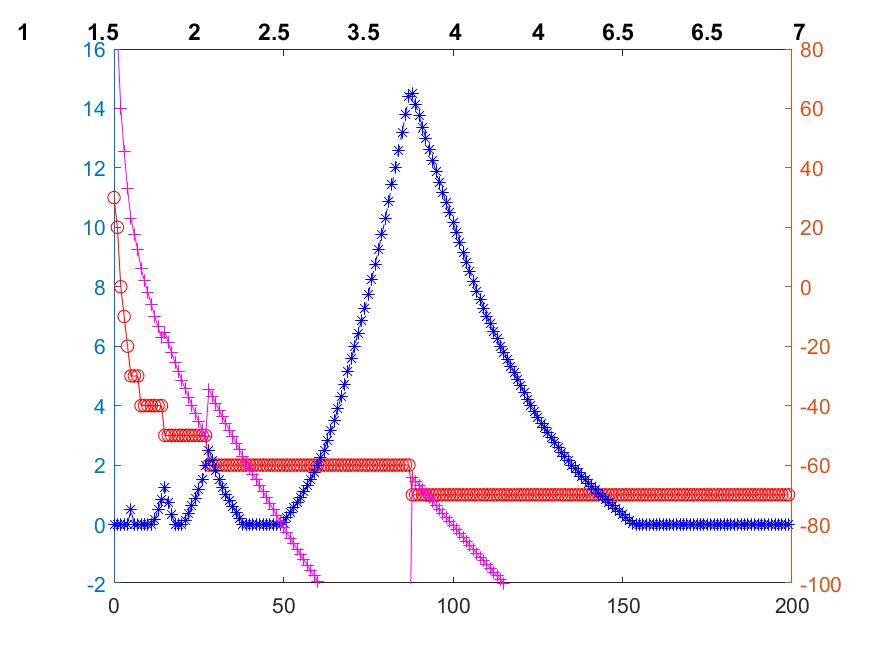
\includegraphics[width=0.7\linewidth]{Figures/Image30}  %插入的图,包括JPG,PNG,PDF,EPS等,放在源文件目录下
	\caption{this is a figure.}  %图片的名称
	\label{fig:mcmthesis-logo}   %标签,用作引用
\end{figure}


\begin{pf}[Theorem 1]

For convenience of expression, we set the setup cost as $S_{1},S_{2}, \dots ,S_{n}$ at interval points while the number of machine changes.
And $S_{i}$ denotes the setup cost when the machine number changes from $i$ to $i-1$, especially, $S_{1}$ denotes the least setup cost when machine number is $1$ and the corresponding subsidy is $0$.
We have the equality

\begin{displaymath}
  S_{1}=S_{2}+\cdots+S_{n}=\sum_{i=2}^n S_i.
\end{displaymath}

Notice that

\begin{displaymath}
  (n-1) \sum_{s \in S \setminus\{V\} } \rho_s \geq
  \sum_{k\in V}\sum_{s \in S \setminus\{V\}:k \in s} \rho_s = n.
\end{displaymath}

The left side of the inequality means for every $\rho_s$ can appear at most $(n-1)$ times, so we should know that if and only if for every $\rho_s > 0$ appears $(n-1)$ times the quality holds.That is to say, the coalitions which contains $(n-1)$ players are all maximally unsatisfied coalitions. Then we have $n \choose n-1$ equalities.
\[
\begin{cases}
 \alpha_1+\alpha_2+ \cdots+\alpha_{n-1} & = x_1 \\
 \alpha_1+\alpha_3+ \cdots+\alpha_n & = x_2 \\
 \quad   \vdots        &\vdots\\
 \alpha_2+\alpha_3+ \cdots+\alpha_n & = x_n.
\end{cases}
\]

Add these $n$ equations together, and we can get

\begin{equation*}
  (n-1)(\alpha_1+\alpha_2+ \cdots+\alpha_n)=\sum_{i=1}^{n}x_i
\end{equation*}

As we know, $x_1,x_2,\dots,x_n$ can be expressed as follows:

\[
\begin{cases}
x_1 = S_0 + (n-1)t_1 + (n-2)t_2 + &\cdots + t_{n-1} \\
x_2 = S_0 + (n-1)t_1 + (n-2)t_3 + &\cdots + t_{n-1} \\
\quad   \vdots        &\vdots\\
x_n = S_0 + (n-1)t_2 + (n-2)t_3 + &\cdots + t_{n}
\end{cases}
\]

According to SPT rule, we can obtain the equality
$c(V)=\alpha_1+\alpha_2+\cdots+\alpha_n=S_0+nt_1+(n-1)t_2+\dots+t_n$
By replacing $x_1,x_2,\dots,x_n$ together with the expression of $c(V)$, we can get a equality only with $S_0,x_1,x_2,\dots,x_n$.

Finally, we can obtain $S_0 = \sum_{k=1}^n (n-k)t_k$.
\end{pf}

\section{ProofTheorem2}



\section{A more specific example}




\end{document}
